%% This is file `elsarticle-template-1-num.tex',
%%
%% Copyright 2009 Elsevier Ltd
%%
%% This file is part of the 'Elsarticle Bundle'.
%% ---------------------------------------------
%%
%% It may be distributed under the conditions of the LaTeX Project Public
%% License, either version 1.2 of this license or (at your option) any
%% later version.  The latest version of this license is in
%%    http://www.latex-project.org/lppl.txt
%% and version 1.2 or later is part of all distributions of LaTeX
%% version 1999/12/01 or later.
%%
%% Template article for Elsevier's document class `elsarticle'
%% with numbered style bibliographic references
%%
%% $Id: elsarticle-template-1-num.tex 149 2009-10-08 05:01:15Z rishi $
%% $URL: http://lenova.river-valley.com/svn/elsbst/trunk/elsarticle-template-1-num.tex $
%%
\documentclass[preprint,12pt]{elsarticle}

%% Use the option review to obtain double line spacing
%% \documentclass[preprint,review,12pt]{elsarticle}

%% Use the options 1p,twocolumn; 3p; 3p,twocolumn; 5p; or 5p,twocolumn
%% for a journal layout:
%% \documentclass[final,1p,times]{elsarticle}
%% \documentclass[final,1p,times,twocolumn]{elsarticle}
%% \documentclass[final,3p,times]{elsarticle}
%% \documentclass[final,3p,times,twocolumn]{elsarticle}
%% \documentclass[final,5p,times]{elsarticle}
%% \documentclass[final,5p,times,twocolumn]{elsarticle}

%% The graphicx package provides the includegraphics command.
\usepackage{graphicx}
%% The amssymb package provides various useful mathematical symbols
\usepackage{amssymb}
%% The amsthm package provides extended theorem environments
%% \usepackage{amsthm}

%% The lineno packages adds line numbers. Start line numbering with
%% \begin{linenumbers}, end it with \end{linenumbers}. Or switch it on
%% for the whole article with \linenumbers after \end{frontmatter}.
\usepackage{lineno}
\usepackage{float}
\usepackage{siunitx}
\DeclareSIUnit\rpm{rpm}
\usepackage{hyperref}
\usepackage{caption}
\usepackage{amsmath}
\makeatletter
\def\ps@pprintTitle{%
 \let\@oddhead\@empty
 \let\@evenhead\@empty
 \def\@oddfoot{}%
 \let\@evenfoot\@oddfoot}
\makeatother

%% natbib.sty is loaded by default. However, natbib options can be
%% provided with \biboptions{...} command. Following options are
%% valid:

%%   round  -  round parentheses are used (default)
%%   square -  square brackets are used   [option]
%%   curly  -  curly braces are used      {option}
%%   angle  -  angle brackets are used    <option>
%%   semicolon  -  multiple citations separated by semi-colon
%%   colon  - same as semicolon, an earlier confusion
%%   comma  -  separated by comma
%%   numbers-  selects numerical citations
%%   super  -  numerical citations as superscripts
%%   sort   -  sorts multiple citations according to order in ref. list
%%   sort&compress   -  like sort, but also compresses numerical citations
%%   compress - compresses without sorting
%%
%% \biboptions{comma,round}

% \biboptions{}



\begin{document}

\begin{frontmatter}

%% Title, authors and addresses

\title{\textbf{Design and Analysis of NASA's Martian Helicopter: Ingenuity}}

%% use the tnoteref command within \title for footnotes;
%% use the tnotetext command for the associated footnote;
%% use the fnref command within \author or \address for footnotes;
%% use the fntext command for the associated footnote;
%% use the corref command within \author for corresponding author footnotes;
%% use the cortext command for the associated footnote;
%% use the ead command for the email address,
%% and the form \ead[url] for the home page:
%%
%% \title{Title\tnoteref{label1}}
%% \tnotetext[label1]{}
%% \author{Name\corref{cor1}\fnref{label2}}
%% \ead{email address}
%% \ead[url]{home page}
%% \fntext[label2]{}
%% \cortext[cor1]{}
%% \address{Address\fnref{label3}}
%% \fntext[label3]{}


%% use optional labels to link authors explicitly to addresses:
%% \author[label1,label2]{<author name>}
%% \address[label1]{<address>}
%% \address[label2]{<address>}

\author{Liz George, Drishika Nadella, Tarun Hegde, Chandran Nandkumar,Jai Mandal, Johns Jaison, Kriti Shukla, Aditya Shrikhande, Samarth Prabhu}

\address{National Institute of Technology Karnataka, Surathkal}

\begin{abstract}
%% Text of abstract
NASA has designed an experimental helicopter named Ingenuity, intended to be a technology demonstrator to assess the feasibility of conducting aerial exploration of other planets/moons in the solar system with atmospheres, such as Venus, Titan or further exploration of Mars. This helicopter is part of the Mars 2020 Perseverance Rover exploration suite, due to be launched in July 2020 and expected to arrive at Mars by February 2021. This project is intended to study the design and analysis of the Martian helicopter Ingenuity from a theoretical perspective. The model is designed on CATIA and static structural analysis is performed on the design to determine the rotor blade's Von Mises stress and deformation. The blades' movement is simulated on Gazebo, a robotics simulator.

\end{abstract}

\begin{keyword}
NASA \sep Mars \sep Ingenuity \sep Design \sep Static structural analysis \sep Von Mises \sep Deformation
%% keywords here, in the form: keyword \sep keyword

%% MSC codes here, in the form: \MSC code \sep codehttps://www.overleaf.com/project/5ee65878df862a000187995c
%% or \MSC[2008] code \sep code (2000 is the default)

\end{keyword}

\end{frontmatter}

\begin{table}[H]
  \begin{center}
    \caption*{\textbf{Authors' Details}}
    \begin{tabular}{c|c|c}
      \textbf{Name} & \textbf{Roll Number} & \textbf{NITK email ID}\\
        & &  \textbf{(id.rollnumber@nitk.edu.in)}\\
      \hline
      Liz George & 181ME241 & lizgeorge\\
      Drishika Nadella & 181ME222 & drishikanadella\\
      Tarun Hegde & 181ME280 & tarun\\
      Chandran Nandkumar & 181ME217 & chandrannandkumar\\
      Jai Mandal & 181ME232 & jai\\
      Kriti Shukla & 181ME239 & kriti\\
      Johns Jaison & 181ME234 & johns\\
      Aditya Shrikhande & 181ME204 & aditya\\
      Samarth Prabhu & 181ME272 & samarthprabhu\\
      
      
    \end{tabular}
  \end{center}
\end{table}





\tableofcontents
\bigskip
\hrule
%% main text
\section{Introduction}
\label{S:1}


Imagine a shoe-box sized device, with blades a few feet long, whizzing to life after charging for a full Sol (a Mars solar day) on Mars. It then flies ahead of a rover to search for hazards and targets of interest and help plan the best driving route for Mars rovers. It flies for a few minutes a day and then returns to the rover where it will spend the day recharging its solar-powered batteries.\par
This device is aptly named Ingenuity or Mars helicopter and is planned for deployment in 2021 from the Perseverance rover as part of the Mars 2020 mission.\par
This helicopter is meant to be a technology demonstrator, and its main task is to image the surface in a higher resolution than orbiting spacecraft are capable of and act as a scout and search for areas of interest for current and future rover missions. If this mission is a success, then perhaps future exploration missions could include larger helicopters as standalone exploratory instruments or even as companions to manned missions.\par

\subsection{\textbf{Background}}

In 1971 the Soviet space program had a major success by putting the first spacecraft into Martian orbit and touching a lander vehicle down on its surface. The Mars 3 orbiter returned eight months of data that revealed much about the planet's topography, atmosphere, weather, and geology. Though the mission's lander was able to touch down on the surface, it returned data for only about 20 seconds before it went dark.\par
Since then, there have been numerous missions to mars including NASA's Mariner 9, Viking 1 and 2 (a pair of orbiter/lander missions which reached Mars in 1976), Mars Pathfinder mission (launched in 1996) , NASA's Mars Global Surveyor (which has orbited the planet since March 1999 on a mission to map and study the planet's entire surface) and Mars exploration rovers Spirit and Opportunity (which reached opposite sides of Mars in January 2004).\par
Now, NASA is sending a light, autonomous rotorcraft, named the Mars Helicopter, to demonstrate the practicability of heavier-than-air vehicles on Mars and get a panorama of the red planet. The atmosphere of Mars is 100 times thinner than that of Earth and flying a helicopter in that kind of air could be gruelling. However, the agency, which has been working on this idea since 2013, has made all the necessary innovations in the design of its Martian helicopter to attempt the flight.\par

\subsection{\textbf{Motivation}}

Understanding whether life exists elsewhere in the Universe beyond Earth is a fundamental question of humankind. Mars is an outstanding place to investigate this question because it is the most similar planet to Earth in the Solar System. There is substantiation that indicates that Mars was once full of water, warmer and had a thicker atmosphere, offering a possibly livable environment. Sending people to Mars is 'the next giant leap for mankind'. This mission will begin huge developments in all kinds of areas, such as solar energy, food production, innovative housing development and the advancement of medical technology.\par
If helicopter flights on Mars become achievable, future vehicles could rake through the Martian landscape for cliffs, investigate cavernous craters, and descend into undiscovered caves dotting the landscape of Mars. One day, it may be viable to ferry payloads from one human outpost to another on Mars, utilizing technology developed with the help of the Martian helicopter Ingenuity. \par

\section{Design}
\label{S:2}

Mars’ average atmospheric pressure on its surface is only 0.6\% ($\sim 610$Pa) of the pressure at sea level on Earth and thus poses several challenges to performing powered flight. Due to the extremely thin atmosphere and lack of adequate power sources, winged flight is out of the question right away. A helicopter design was chosen due to its compactness and relative ease of operation in Martian conditions. 

A helicopter generates lift by using its rotors to push down air, in turn lifting the body of the chopper up.
Since the atmosphere on Mars is much thinner than on Earth, the rotors of Ingenuity are quite large and wide relative to the size of the body, having a higher inherent rotational pitch (angle of attack of the rotor blade). 

\begin{figure}[h]
\centering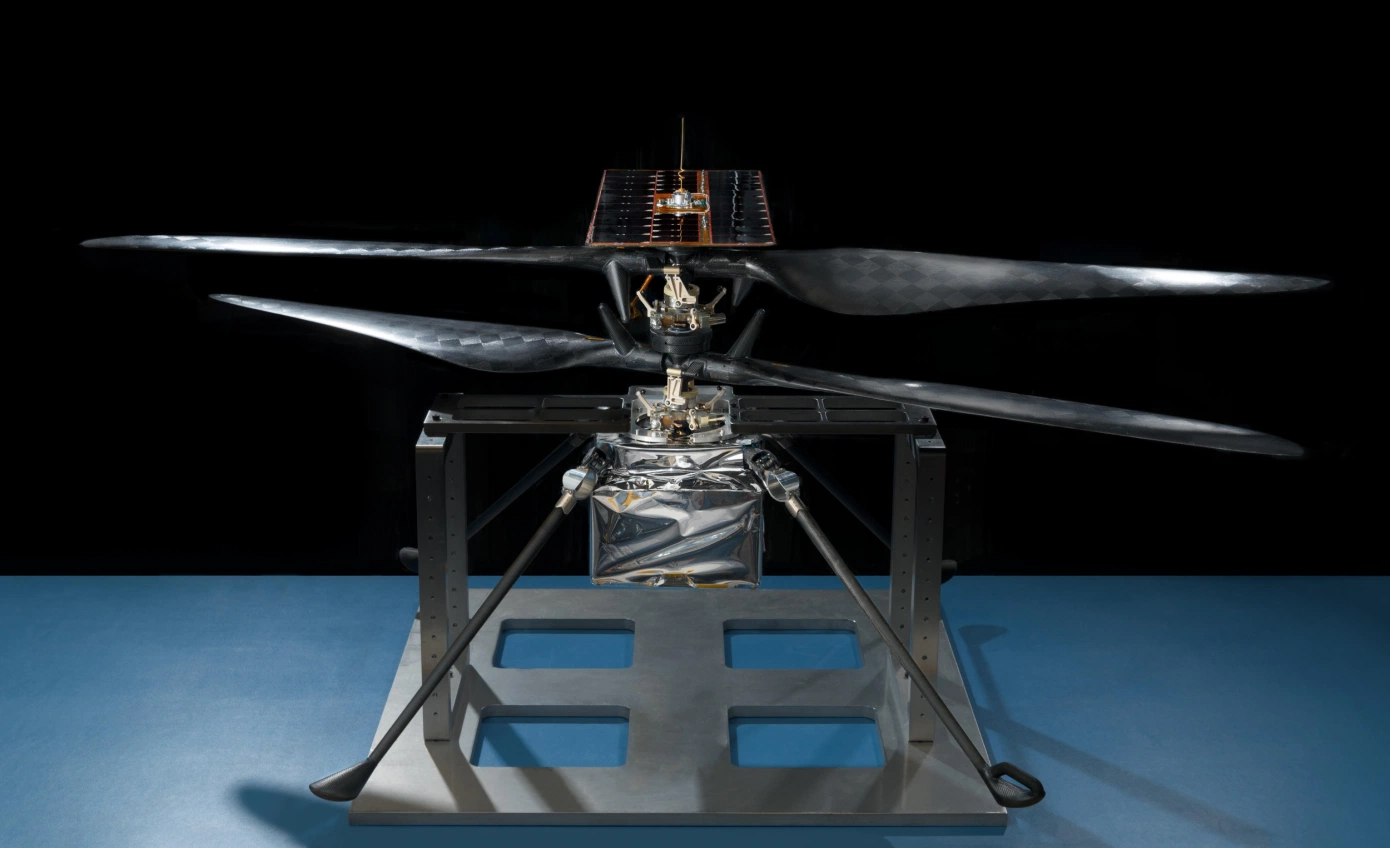
\includegraphics[width=0.4\linewidth]{Ingenuity.png}
\caption{An experimental prototype of Ingenuity designed by NASA}
\end{figure}


When launching payloads into space, the shape, size and weight of the instruments is heavily constrained as it is very expensive to launch heavy payloads into orbit, let alone to Mars. This calls for several design optimizations with regards to the helicopter. \par

The spacecraft has a cube shaped chassis of 14x14x14 cm, which contains all of the spacecraft’s scientific payload, flight control systems, batteries and navigation systems.
 It has a height of about 80cm, both blades have a combined diameter of 1.2m and the whole spacecraft weighs about 1.8kg on Earth or 684g on Mars (Mars only has around 38\% of the gravitational force of Earth).\par

To reduce the spacecraft’s footprint, NASA opted for a coaxial rotor design instead of a traditional tail rotor or quad copter design. The coaxial rotors rotate in opposite directions to each other, which cancels out the counter torque produced by each blade, ensuring stability of the whole spacecraft. \par

Typically, helicopters on Earth have rotor speeds of about 500 rpm, but due to the thinness of the Martian atmosphere, Ingenuity’s rotor blades need to spin at 2400 rpm (about 5 times faster than on Earth) despite the weight reduction due to Mars’ weaker gravity, to generate sufficient lift. \par

Ingenuity’s rotor blades are made up of a foam core, and covered by several layers of carbon fibre, making them very lightweight; each weighing in at about 35g. These blades are able to provide for a flight time of about 90 seconds at a time. \par

Since the blades need to be very long to generate sufficient lift, a quad-copter design was ditched in favor of a coaxial design due to size constraints. A coaxial design also offers better lift, because the top rotor acts as a funnel that sucks air in and the bottom rotor, pushes down the column of air to generate a considerable amount of stable lift. Since the blades spin at a much faster rate than they need to on Earth, the rotation speed needs to be carefully monitored and set so that the tip speed does not exceed the speed of sound. \par

To perform structural analysis on Ingenuity, the design model was created on CATIA (shown in Figure 2). Its dimensions are listed in Table 1\par

\begin{figure}[H]
\centering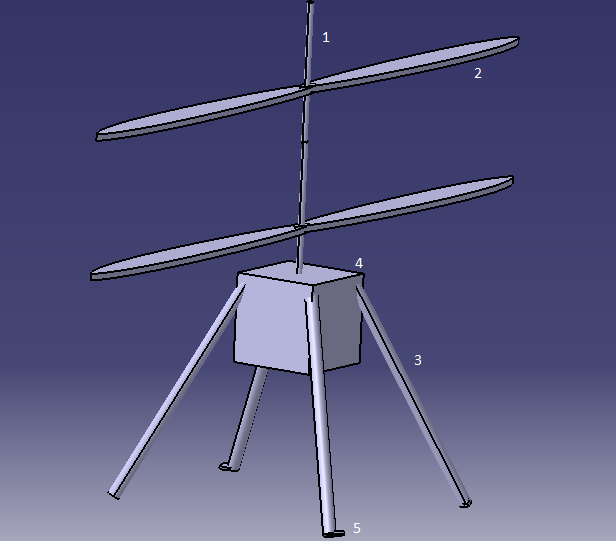
\includegraphics[width=0.4\linewidth]{Ingenuity cad model.png}
\caption{A basic CAD model of the prototype of Ingenuity.}
\end{figure}


\begin{table}[H]
\centering
\begin{tabular}{c|c}
\hline
\textbf{Part Number} & \textbf{Dimensions(mm)}\\
\hline
1 & Length - 220, Diameter - 50 \\
2 & Blade length - 600, Thickness - 5 \\
3 & Length - 400, Diameter - 20\\
4 & Length - 140, Breadth - 140, Height - 140\\
5 & Length - 50, Thickness - 3\\
\hline
\end{tabular}
\caption{Dimensions of the model}
\end{table}

\section{Analysis}
\label{S:3}

\subsection{\textbf{Structural Analysis}}
\subsubsection{\textbf{Calculations for pre-analysis}}

\begin{enumerate}
\item Formula to calculate centrifugal force 
\begin{equation}
    mv^2/R = m(2^2\pi^2N^2R^2)/3600R
    \label{eq:cent}
\end{equation}
N = \SI{2400}{rpm}\\
R = \SI{0.6}{\metre}\\
m = \SI{0.02}{\kilogram}\\
Substituting the values in Equation \ref{eq:cent},\\
Centrifugal force = \SI{757}{\newton}\\

\item Lift(L) is given by the following equation\\
 \begin{equation}
    L = \rho v^2AC_L /2
    \label{eq:lift}
\end{equation}
A = \SI{0.0273}{\metre\squared}\\
$\rho$ = \SI{0.02}{\kilogram\per\metre\cubed} (Martian atmosphere density)\\
v = (2$\pi$N/60)*R = \SI{150.7962}{\metre\per\second}\\
Lift coefficient, $C_L$ = 0.5\\
Substituting the values in Equation \ref{eq:lift}, we get\\
L = 6.14*$C_L$ = \SI{3.07}{\newton}
\end{enumerate}
\subsubsection{\textbf{Steps involved in pre-analysis}}
\begin{itemize}
    \item First step involved calculation of lift which came up to 3N
    \item This was then distributed over the blade such that maximum occurs on the tip and 0 at the fixed end. This was a uniformly varying load.
    \item Then due to rotation, moment of rotation was also added about the fixed end which came up to \SI{1.2}{\newton\metre}
    \item Centrifugal force is added to the blade. 
    \item An analysis was performed on ANSYS
\end{itemize}
Everything except the $C_L$ is direct. To find the lift coefficient for the blade in a Martian atmosphere we referred to papers that dealt with this exact problem.
In the paper, they took Reynolds number as 11,000, Mach Number as 0.21 and used the NACA0012 airfoil (open source airfoil) and estimated the $C_{L_{max}}$ as 0.5 through wind tunnel testing.

This is the graph of coefficient vs angle of attack in the paper
\begin{figure}[H]
\centering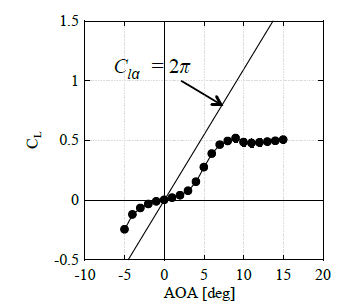
\includegraphics[width=0.69\linewidth]{graph of coefficient.png}
\caption{Graph depicting Lift coefficient vs Angle of Attack}
\end{figure}
Density of Rotor Blade: \SI{72.574}{\kilogram\per\metre\cubed}\\
Software used: ANSYS 16.0\\
Material used: Carbon fibre with foam core\\

The analysis shown above is the structural analysis of the rotor blades of Ingenuity.

We considered the lift and moment about the fixed support as the key contributors to load when analysing the rotor blades. The lift was varied uniformly from the fixed support point to the tip of the rotor blade.

\subsubsection{\textbf{Results}}
{The end result of analysis on ANSYS can be seen in the images given below
\begin{figure}[H]
\centering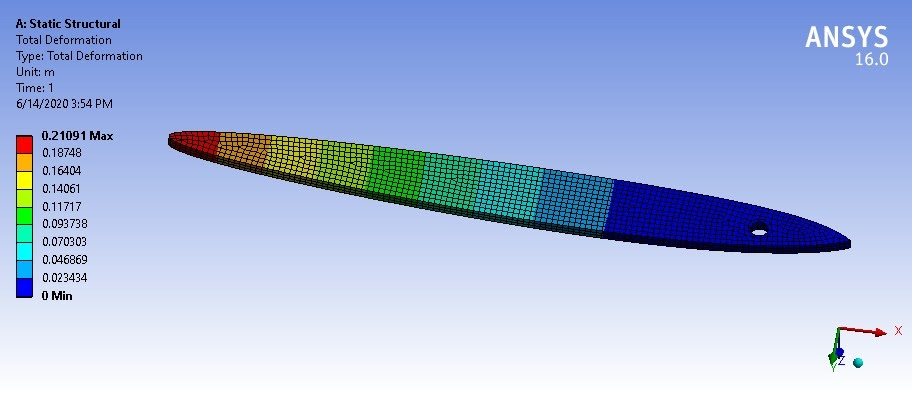
\includegraphics[width=1.0\linewidth]{rotor mesh 1.png}
\caption{Total Deformation contour plotted on ANSYS}
\bigskip
\centering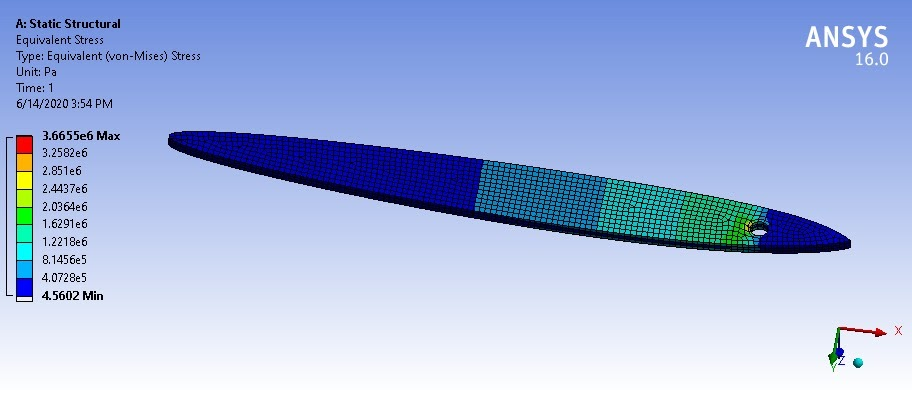
\includegraphics[width=1.0\linewidth]{rotor mesh 2.jpeg}
\caption{Equivalent Stress contour plotted on ANSYS}
\smallskip
\end{figure}
As we can see in the images above, the maximum deformation is \SI{0.21091}{\metre} and the 
von Mises stress comes about to be a maximum of \SI{3.6655}{\pascal}.

As we can observe from the structural analysis above, the deflection is not considerably large which is ideal for the design and serves to prove that the design is practical and can be implemented without any damage to the rotor blades.\par
As we can see in the images above, von Mises stresses and the total deformation is rather small, making them ideal for low atmosphere flight.}

\subsection{\textbf{Electronic Simulation}}
The simulation of Ingenuity’s rotor blades moving was created for better visualization of the helicopter flying. This was done using Gazebo, an open source 3D robotics simulator.Figure 7 shows the circuit for the DC motor that spins the helicopter blades. It was simulated on Tinkercad using an Arduino board.
\begin{figure}[H]
\centering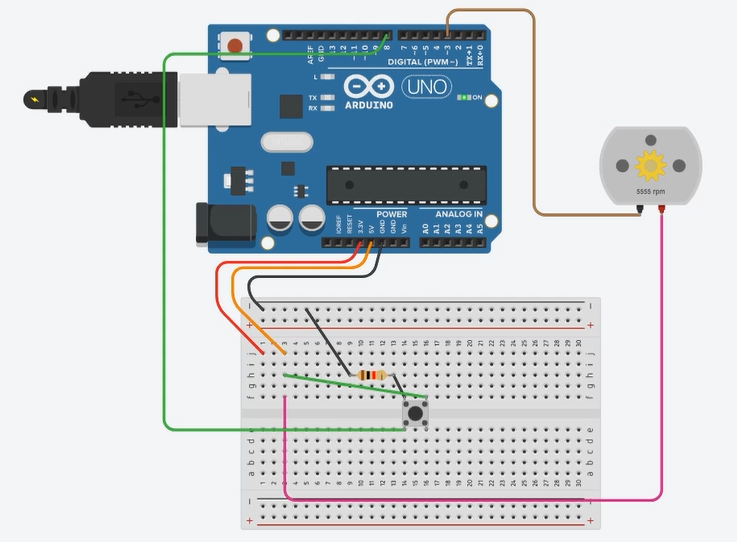
\includegraphics[width=0.69\linewidth]{dc motor ckt.png}
\caption{DC motor circuit}
\end{figure}
Figure (6) shows the helicopter blades being rotated using Gazebo.
\begin{figure}[H]
\centering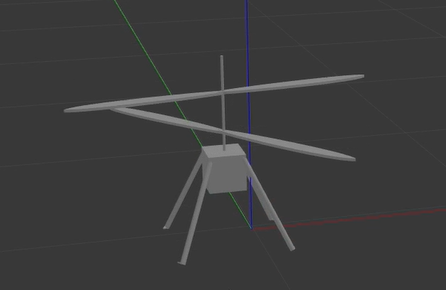
\includegraphics[width=0.69\linewidth]{gazebo sim.png}
\caption{Simulation of the rotation of the co-axial blades on Ingenuity using Gazebo}
\end{figure}

\section{\textbf{Conclusion}}
At the end of the project, the team believes that this project has motivated the authors and widened their research capabilities. 
Ingenuity, the Martian helicopter, planned for deployment in 2021 from the Perseverance Rover is another big step towards space exploration, that can take us one step closer to establishing ourselves as an interplanetary species. The success of Ingenuity can inspire future aerial missions.

\section*{\textbf{Acknowledgement}}
\addcontentsline{toc}{section}{Acknowledgement}
The authors would like to express their gratitude to the Department of Mechanical Engineering, NITK for providing us the opportunity to be working on a project which requires the complete use of our practical knowledge and more.\\
The authors would like to thank Professors Sharnappa J and Subhaschandra Kattimani for their constant support and guidance without which this project would have been impossible.\\ 
The authors would also like thank Dassault Systèmes SE, Autodesk Inc., and the Open Source Robotics Foundation, for providing the software used for the design, analysis and simulation in the project\\
We, the authors, express our heartfelt thanks to everyone involved for their efforts.\\

\section*{\textbf{References}}
\addcontentsline{toc}{section}{References}
\begin{enumerate}
    \item Koning, W.J., Romander, E.A., Johnson, W. (2018). Low Reynolds Number Airfoil Evaluation for the Mars Helicopter Rotor.\footnote{\href{https://rotorcraft.arc.nasa.gov/Publications/files/Koning_Romander_Johnson_Low_Reynolds_Number_Airfoil_Evaluation_FINAL_ARC.pdf}{Link to the paper}} 
    \item NASA's Mars Exploration Program\footnote{\url{https://mars.nasa.gov}}
    \item CalTech Jet Propulsion Laboratory\footnote{\url{https://jpl.nasa.gov}}
    \item Wikipedia\footnote{\url{https://wikipedia.org}}
    \item Veritasium on YouTube\footnote{\url{https://youtube.com/Veritasium}}
    \item Mars One\footnote{\url{https://mars-one.com}}
    \item National Geographic Magazine\footnote{\url{https://nationalgeographic.com}}
\end{enumerate}


\end{document}